\documentclass[10 pt,usenames,dvipsnames, oneside]{article}
\usepackage{../../../modelo-ensino-medio}



\begin{document}

\begin{center}
  \begin{minipage}[l]{3cm}

\includegraphics[width=2cm]{logo}    
\end{minipage}\hfill
\begin{minipage}[r]{.8\textwidth}
 {\Large \scshape Atividade: Cobrindo circunferências com seus raios}  
\end{minipage}
\end{center}
\vspace{.2cm}

\ifdefined\prof
%Habilidades da BNCC
% \begin{objetivos}
% \item 
% \end{objetivos}

%Caixa do Para o Professor
\begin{goals}
%Objetivos específicos
\begin{enumerate}
\item Introduzir ao aluno uma nova forma de se mensurar ângulos na circunferência, tomando como unidade de medida, um arco de medida igual ao raio da mesma.
\end{enumerate}

\tcblower

%Orientações e sugestões
Os itens \titem{b)} e \titem{c)} pretendem convencer o aluno de que, independente do tamanho da circunferência, essa nova unidade de medida corresponde a um mesmo valor em graus, valor este aproximadamente $57^{\circ}$, o que permitirá estabelecer uma primeira correspondência entre essas duas formas de medir ângulos. 

Ao longo da atividade, o aluno poderá adotar diferentes estratégias, como dividir os $360$ graus de uma volta inteira pela medida do ângulo central ou ainda ir colando outros pedaços de barbante sobre o contorno da circunferência para verificar. Cuide para que eles adotem as próprias estratégias e que compartilhem uns com os outros. Nesta atividade, caso prefira, pode-se também desenhar diferentes circunferências usando o compasso, substituindo os objetos redondos.
\end{goals}

\bigskip
\begin{center}
{\large \scshape Atividade}
\end{center}
\fi

Vamos propor agora uma atividade para você fazer com os seus colegas na sala de aula. Se organizem em duplas ou grupos e sigam os passos a seguir:
\begin{enumerate}[label=\titem{\arabic*.}, wide, left=0pt]
\item Providencie objetos redondos que você possa levar para a sala de aula (rodinhas de carrinho de brinquedo, copos, garrafas, tampas de potes e panela, etc);
\item Use esses objetos para desenhar circunferências numa folha suficientemente grande, contornando-as com um lápis;
\item Determine o centro dessas circunferências. Para isso, tome três pontos sobre a circunferência e trace as mediatrizes de dois segmentos distintos com extremidades nesses pontos. O encontro entre essas mediatrizes é o centro da circunferência;
\item Meça o raio dessas circunferências;
\item Para cada uma das circunferências, corte um pedaço de barbante que tenha essa medida e ajuste-o sobre a circunferência, colando-o no papel.
\end{enumerate}

\begin{figure}[H]
\centering

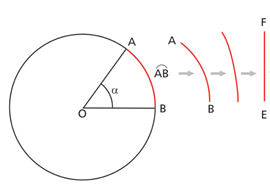
\includegraphics[width=.4\linewidth]{trigonometricas37}
\end{figure}

\begin{enumerate}
\item Qual o nome do objeto geométrico equivalente à parte das circunferências coberta pelo barbante?
\item A partir de cada extremidade dos pedaços de barbante colados sobre cada circunferência, trace dois segmentos que unam as extremidades dos barbantes ao centro de cada circunferência. Meça os ângulos centrais que ficam assim determinados em cada circunferência. Qual a medida do ângulo central encontrada em cada uma delas?
\item Compare a sua resposta do item \titem{c)} com as de outras duplas ou grupos de sua turma. Há algo que você consegue notar nos valores obtidos?
\item Quantas vezes o raio da circunferência cabe no comprimento da mesma?
\item É possível cobrir toda a circunferência com uma quantidade inteira de segmentos com medida igual à do seu raio? Se sim, diga quantos segmentos são necessários; se não, estime o valor da fração do raio do círculo correspondente ao pedacinho que ficou descoberto.
\end{enumerate}

\ifdefined\prof
\begin{solucao}

\begin{enumerate}
\item Arco
\item A medida do ângulo será, o valor em graus de 1 radiano,
isto é, aproximadamente $57^{\circ}$.
\item Os valores serão muito próximos, com pequenas variações em virtude de erros de medição.
\item $6$
\item Não é possível cobrir a circunferência com uma quantidade inteira de raios, visto que o seu comprimento é o resultado da multiplicação do raio por um número irracional: $C =(2\pi)r\approx6{,}28r = 6r + 0{,}28r$.

Logo, a parte que fica descoberta, referida no enunciado, corresponderá a um valor aproximado de 0,28 vezes a medida do raio. 
\end{enumerate}

\end{solucao}
\fi

\end{document}